% TODO: Check "islands set" vs "island set".
% TODO: Avoid "mapped to infinity", because it means "undefined".
\chapter{Stationary States Classification Within Symbolic Dynamics Framework}

\section{Objections}

In this chapter we describe an approach that is used further in order to classify all stationary state of one-dimensional GPE that are described by the stationary states equation:
\begin{equation}
	u_{xx} + Q(x) u + P(x) u^3 = 0.
	\label{eq:stationary}
\end{equation}
Here and after we assume $Q(x)$, $P(x)$ to be periodic functions of the same period $L$: $Q(x + L) = Q(x)$, $P(x + L) = P(x)$ which is quite typical for different physical applications.
We also assume functions $Q(x)$, $P(x)$ to be at least piece-wise continuously differentiable.
That allows us to split the whole real axis $\mathbb{R}$ into separate intervals where the corresponding Cauchy problem correctly defined and a solution for any initial conditions exists and is unique within each such interval.

Our classification approach is based on the technique proposed in the work \cite{AlfimovAvramenko}.
In \cite{AlfimovAvramenko} authors show that presence of a large number of singular solutions families allows to classify all remaining bounded solutions within a symbolic dynamics framework.
That leads us to another important requirement, function $P(x)$ must {\it changes its sign along the period} $L$.
As we saw in the previous chapter such fact guarantees the existence of singular solution families that in its turn becomes a foundation of the technique and makes the announced approach even possible.

Goal of this chapter is to provide a stationary states classification framework and point out the boundaries of its application.
Core idea is the following.
We define a Poincar\'e map $\mathcal{P}$ for the stationary states equation \eqref{eq:stationary}.
Since function $P(x)$ alternates its sing, Poincar\'e map $\mathcal{P}$ and an inverse map $\mathcal{P}^{-1}$ cannot be defined on the whole phase plane, instead they are defined on some phase plane subset.
Studying the domains of maps $\mathcal{P}$, $\mathcal{P}^{-1}$ is a crucial aspect of the proposed approach.
We determine conditions which allow to conclude that Poincar\'e map acts on the defined set as a kind of the {\it horseshoe map} \cite[Chapter 5]{GuekenheimerHolmes}.
Domains of the higher order maps $\mathcal{P}^2,~\mathcal{P}^3, \dots$ and domains of the inverse maps $\mathcal{P}^{-2},~\mathcal{P}^{-3}, \dots$ can be obtained by the refinement of the initial area.
Finally if some conditions are met and we can conclude that there exists one-to-one correspondence between all bounded solution of the equation \eqref{eq:stationary} and a points set on the phase plane which is a result of the above mentioned refinement.
That is what we call singular solution elimination method.

The presence of the horseshoe map structure allows us for each bounded solution uniquely specify a bi-infinite symbolic sequence over some alphabet (finite or even infinite) and such correspondence is also bijective.
We refer to the result bi-infinite sequence as {\it solution code} and the overall process as {\it solutions coding}.
Such coding, if possible, provides a complete picture of the bounded solutions family for the equation \eqref{eq:stationary} that can be highly demanded in different physical applications which involves Gross-Pitaevskii equation with both periodic potential and periodic pseudopotential.

\section{Geometry of the Poincar\'e Map}

First of all let's introduce several definitions which describe basic structures and their relationships that are in the core of the overall further narration.

\subsection{Poincar\'e Map}

Since we consider functions $Q(x)$, $P(x)$ to be $L$-periodic let's introduce the Poincar\'e map associated with the period $L$ of the equation \eqref{eq:stationary}.
Define the Poincar\'e map $\mathcal{P}: \mathbb{R}^2 \to \mathbb{R}^2$ in the following manner:
\begin{equation}
	\mathcal{P} \begin{pmatrix} u_0 \\ u_0' \end{pmatrix}
	= \begin{pmatrix} u_L \\ u_L' \end{pmatrix},
\label{eq:poincare-map}
\end{equation}
where $u_L = u(L)$, $u_L' = u'(L)$, and $u(x)$ is a solution of the equation \eqref{eq:stationary} with initial conditions $u(0) = u_0$, $u'(0) = u_0'$.
Poincar\'e map by itself is an {\it area-preserving diffeomorphism}.
Obviously, and as we mentioned above, Poincar\'e map $\mathcal{P}$ and its inverse $\mathcal{P}^{-1}$ may not be defined on the whole plane $(u, u')$ of initial conditions.
Denote by $\mathscr{U}_L^+$ the domain of the map $\mathcal{P}$, and denote by $\mathscr{U}_L^-$ the domain of the map $\mathcal{P}^{-1}$ correspondingly.
Also define a set $\mathscr{U}_L$ as an intersection of the two above mentioned sets: $\mathscr{U}_L = \mathscr{U}_L^+ \cap \mathscr{U}_L^-$.

It obviously follows from the definitions of $\mathscr{U}_L^{\pm}$ that $\mathcal{P}(\mathscr{U}_L^+) = \mathscr{U}_L^-$.
Indeed any point $\vb{p} \in \mathscr{U}_L^+$ has $\mathcal{P}$-image $\vb{q}$.
Then $\vb{q}$ has $\mathcal{P}$-pre-image, therefore $\vb{q} \in \mathscr{U}_L^-$.
On the other hand if $\vb{q} \in \mathscr{U}_L^-$ then $\vb{q}$ has $\mathcal{P}$-pre-image $\vb{p}$.
Therefore $\vb{p}$ has $\mathcal{P}$-image and hence $\vb{p} \in \mathscr{U}_L^+$.
Backward statement $\mathcal{P}^{-1}(\mathscr{U}_L^-) = \mathscr{U}_L^+$ is also valid.

We also note here that symmetry in equation \eqref{eq:stationary} naturally produces symmetry in $\mathcal{U}_L^{\pm}$ sets.
For example we can prove the following important statement.

\begin{proposition}
	Let functions $Q(x)$, $P(x)$ are even, then 
	\begin{eqnarray}
		&& \mathcal{P}(\mathscr{U}_L^+) = I (\mathscr{U}_L^+); \label{eq:domain-reflection-forward} \\
		&& \mathcal{P}^{-1}(\mathscr{U}_L^-) = I (\mathscr{U}_L^-), 	\label{eq:domain-reflection-backward}
	\end{eqnarray}
	where map $I$ is a reflection with respect to the $u'$ axis.
\label{prop:domain-reflection}
\end{proposition}
\begin{proof}
	Let's prove statement \eqref{eq:domain-reflection-forward}.
	Consider a point $\vb{q} \in \mathcal{P}(\mathscr{U}_L^+)$.
	By definition of $\mathscr{U}_L^+$ set there is a point $\vb{p} = (u_0, u_0') \in \mathscr{U}_L^+$, such that there exists a solution $u(x)$ of \eqref{eq:stationary} with initial conditions $u(0) = u_0$, $u'(0) = u_0'$, and $\vb{q} = (u(L), u'(L))$.
	Denote by $\widetilde{\vb{p}}$ a reflection $I(\vb{p})$, $\widetilde{\vb{p}} = (-u_0, u_0')$.
	Next we note that equation \eqref{eq:stationary} along with the proposition assumptions on functions $Q(x)$, $P(x)$ admits the variables change $\widetilde{u} = -u$, $\widetilde{x} = -x$ and the form of \eqref{eq:stationary} remains exactly the same.
	It means that $\widetilde{u}(\widetilde{x})$ is also a solution of \eqref{eq:stationary} with initial conditions $\widetilde{u}(0) = -u_0$, $\widetilde{u}'(0) = u_0'$.
	It follows from the introduced variables change that $\widetilde{u}(-L) = -u(L) = -u_L$ and $\widetilde{u}'(-L) = u'(L) = u_L'$.
	Denote this new point by $\widetilde{\vb{q}} = (\widetilde{u}(-L), \widetilde{u}'(-L))$.
	By definition of $\mathcal{P}$ map, $\widetilde{\vb{q}} = \mathcal{P}^{-1}(\widetilde{\vb{p}})$ and hence $\widetilde{\vb{q}} \in \mathscr{U}_L^+$.
	On the other hand $\widetilde{\vb{q}} = (-u_L, u_L') = I(\vb{q})$.
	Finally from $I(\vb{q)} \in \mathscr{U}_L^+$ we get $\vb{q} \in I(\mathscr{U}_L^+)$.
	It's also pretty straightforward to check backward statement $\vb{q} \in I(\mathscr{U}_L^+) \Rightarrow \vb{q} \in \mathcal{P}(\mathscr{U}_L^+)$ and eventually prove the equality \eqref{eq:domain-reflection-forward}.
	Statement \eqref{eq:domain-reflection-backward} can be proven in an identical manner.
\end{proof}

If the conditions of Proposition \ref{prop:domain-reflection} are met one can conclude that $I (\mathscr{U}_L^+) = \mathscr{U}_L^-$ and $I (\mathscr{U}_L^-) = \mathscr{U}_L^+$, so the above mentioned sets are connected with each other with a reflection with respect to the $u'$ axis.

\begin{definition}
	Define an {\bf orbit} as a sequence of points $\{ \vb{p}_n \}$, $\vb{p}_n \in \mathbb{R}^2$ such that $\mathcal{P}(\vb{p}_n) = \vb{p}_{n+1}$.
\label{def:orbit}
\end{definition}

Let $\vb{p}_0$ be a starting point.
Since $\mathcal{P}$ is defined only on the $\mathscr{U}_L^+$ set, the next point $\vb{p}_1$ of the orbit exists only if $\vb{p}_0 \in \mathscr{U}_L^+$.
Moreover for $n > 0$ points $\vb{p}_n$ are consecutive $\mathcal{P}$-iterations of the initial point $\vb{p}_0$.
If at $k$-th iteration $\mathcal{P}^k(\vb{p}_0)$ leaves the $\mathscr{U}_L^+$ set then the orbit cannot be defined for $n > k$.
Similarly for $n < 0$ points $\vb{p}_n$ are consecutive $\mathcal{P}^{-1}$-iterations of $\vb{p}_0$.
Since the $\mathcal{P}^{-1}$ map defined only on the $\mathscr{U}_L^-$ set the iterations may stop after a finite number of steps.
As a consequence not all orbits are bi-infinite.
But bi-infinite orbits are also exists.
For example one can easily specify the bi-infinite orbit of zero points that trivially satisfies the equation \eqref{eq:stationary} and corresponds to its zero solution $u(x) \equiv 0$.

Another interesting observation comes from Proposition \ref{prop:absense-of-singular-solutions}.
If the function $P(x) > 0$ for all $x \in \mathbb{R}$ then all the orbits for the equation \eqref{eq:stationary} are bi-infinite.
From that point of view the case when $P(x)$ changes its sing becomes interesting.
According to Proposition \ref{prop:singular-families} points where $P(x) < 0$ form the families of collapsing solutions.
Such families at their turn sift the set of bi-infinite orbits.
It becomes highly desired, and we'll require it further, that the defined set $\mathscr{U}_L$, produced by the Poincar\'e map $\mathcal{P}$, represents a so-called {\it island set}  \cite{AlfimovAvramenko} (it will be defined soon).
Looking ahead, such structure along with additional properties clearly reveals the horseshoe structure and allows us to formulate and prove all the essential theorems and describe the set of remaining bi-infinite orbits. 

\subsection{Islands Set}

\begin{definition}
	Let $\gamma > 0$ is fixed.
	A continuous function $f(x): \Delta \to \mathbb{R}^2$, $\Delta = [a, b]$ is called $\bm{\gamma}$-{\bf Lipschitz} function if $\forall x_1, x_2 \in \Delta$ the following inequality holds:
	\begin{equation}
		|f(x_1) - f(x_2)| \le \gamma |x_1 - x_2|.
	\end{equation}
\end{definition}

\begin{definition}
	We call {\bf island} an open curvilinear quadrangle $D \subset \mathbb{R}^2$ on the phase plane $(u, u')$ formed by two pairs of nonintersecting monotonic curves $\alpha^{\pm}$, $\beta^{\pm}$, moreover:
	\begin{itemize}
		\item curves $\alpha^{\pm}$ are graphs of monotonic $\gamma$-Lipschitz functions $u' = h_{\pm}(u)$, and a solution of the equation \eqref{eq:stationary} with initial conditions $(u_0, u_0') \in \alpha^{\pm}$ collapses at the point $x = -L$;
		\item curves $\beta^{\pm}$ are graphs of monotonic $\gamma$-Lipschitz functions $u = v_{\pm}(u')$, and a solution of the equation \eqref{eq:stationary} with initial conditions $(u_0, u_0') \in \beta^{\pm}$ collapses at the point $x = +L$;
		\item if the functions $h_{\pm}(u)$ are increasing then $v_{\pm}(u')$ are decreasing, and vice versa, if functions $h_{\pm}(u)$ are decreasing then $v_{\pm}(u')$ are increasing respectively.
	\end{itemize}	
\end{definition}

\begin{remark}
	For convenience hereinafter by monotonically increasing / decreasing function we mean a function that satisfy non-strict inequalities.
	We call function $f(x)$ monotonically increasing if for $x_1 < x_2$, $f(x_1) \le f(x_2)$, and monotonically decreasing if $f(x_1) \ge f(x_2)$.
\end{remark}

To emphasise the fact that Lipschitz constant $\gamma$ must be predefined we also refer to the island as \bm{$\gamma$}-{\bf island}.
We also say that points from the island boundaries are {\it mapped to infinity} by $\mathcal{P}$ ($\beta^{\pm}$ boundaries) or $\mathcal{P}^{-1}$ ($\alpha^{\pm}$ boundaries), since the corresponding solution to the Cauchy problem with initial conditions in that points collapse exactly in the points $x = \pm L$.

\begin{remark}
	If $D$ is a $\gamma_1$-island and $\gamma_2 > \gamma_1$	then $D$ also is a $\gamma_2$-island.
\end{remark}

In our definition of island we explicitly specify its connection with initial equation \eqref{eq:stationary} and collapses of its solutions.
Further we'll see that such connection naturally comes from the dynamics of the $\mathcal{P}$ map for equation of such type.

\begin{remark}
	Solution of the Cauchy problem for the initial conditions at the  intersections of the $\alpha^{\pm}$, $\beta^{\pm}$ curves collapse both in $x = +L$ and $x = -L$ points.
\end{remark}

\begin{definition}
	Let $S$ be a finite or a countable set of indices.
	Define {\bf island set} as a set $\mathcal{D} = \bigcup_{i \in S} D_i$ that represents finite or countable union of disjoint islands.
\label{def:island-set}
\end{definition}

% TODO: What does it mean, mapped to infinity?
\begin{figure}[h]
\centering
	\includegraphics[scale = 1]{pic/islands set}
	\caption{Hypothetical example of an island set $\mathcal{D} = \bigcup_{i \in \{1, 2, 3\}} D_i$ on a plane of initial conditions for the equation \eqref{eq:stationary}. Boundaries of each component are mapped to the infinity by the $\mathcal{P}$ and $\mathcal{P}^{-1}$ maps (solution of the corresponding Cauchy problem is collapses).}
\label{fig:islands-set}
\end{figure}

\subsection{Curves and Strips}

Move on to the definition of h,v-curves and h,v-strips.
Such curves and strips along with theirs transformations are the object of our attentive study.

\begin{definition}
	Let $D$ be an island bounded by curves $\alpha^{\pm}$, $\beta^{\pm}$.
	Consider a curve $\alpha$ that connects the opposite sides $\beta^{\pm}$ of the island $D$. 
	We call such curve {\bf h-curve} if it represents a graph of a monotonic $\gamma$-Lipschitz function $u' = h(u)$ and its monotonicity type coincide with the functions $u' = h_{\pm}(u)$ that correspond to the $\alpha^{\pm}$ boundaries of the island $D$.
	We also call {\bf h-strip} an open subset of the island $D$ bounded by two \emph{h}-curves.
\end{definition}

\begin{definition}
	Similarly consider a curve $\beta$ that connects opposite sides $\alpha^{\pm}$ of an island $D$.
	We call it {\bf v-curve} if it represents a graph of a monotonic $\gamma$-Lipschitz function $u = v(u')$ and its monotonicity type coincide with the functions $u = v_{\pm}(u')$ that correspond to the $\beta^{\pm}$ boundaries of the island $D$.
	In a like manner we call {\bf v-strip} an open subset of the island $D$ bounded by two \emph{v}-curves.
\end{definition}

\begin{remark}
	Island by itself represents a limit case of the h and v strips simultaneously.
\end{remark}

% TODO: Make this figure a bit smaller, use 16 pt. for letters.
\begin{figure}[h]
\centering
	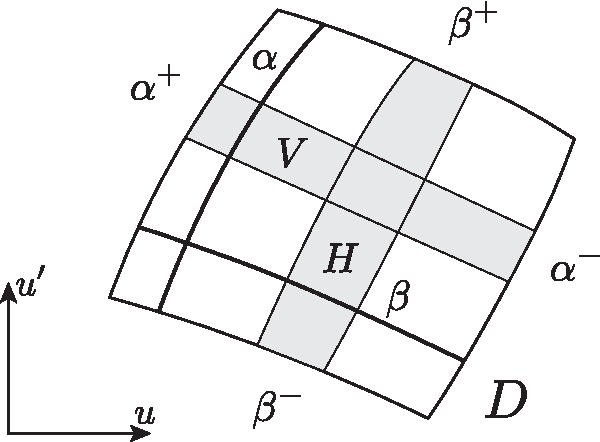
\includegraphics[scale = 1]{pic/curves and strips}
	\caption{An islands $D$ bounded by curves $\alpha^{\pm}$, $\beta^{\pm}$; h-curve $\alpha$, v-curve $\beta$, and two strips: h-strip $H$ and v-strip $V$.}
\label{fig:curves-and-strips}
\end{figure}

All above introduced definitions are illustrated on Figures \ref{fig:islands-set} and \ref{fig:curves-and-strips}.
At last let's define one additional property of island set along with $\mathcal{P}$, $\mathcal{P}^{-1}$ maps.

\begin{definition}
	Let $\mathcal{D}$ be an island set formed by the domains of the $\mathcal{P}$ and $\mathcal{P}^{-1}$ maps that act on this set.
	Consider two islands $D_1, D_2 \in \mathcal{D}$.
	We call the island $D_2$ {\bf forward-reachable} from the island $D_1$ if for any \emph{h}-curve $\alpha \in D_1$ with endpoints lying on the opposite boundaries $\beta_1^{\pm}$ of the island $D_1$ the intersection $\mathcal{P}(\alpha) \cap D_2$ is not empty.
	On the other hand we call the island $D_2$ {\bf backward-reachable} from the island $D_1$ if for any \emph{v}-curve $\beta \in D_1$ with endpoints lying on the opposite boundaries $\alpha_1^{\pm}$ of the island $D_1$ the intersection $\mathcal{P}^{-1}(\beta) \cap D_2$ is not empty.
	Finally we call the island $D_2$ {\bf reachable} from the $D_1$ if it satisfies both forward and backward reachability.
\end{definition}

\begin{remark}
	If an island $D_2$ is forward-reachable from $D_1$ then $D_1$ is backward-reachable from $D_2$ and vice versa.
\end{remark}

\begin{definition}
	We call an island set $\mathcal{D} = \bigcup_{i \in S} D_i$ {\bf complete} if for any $i, j$ island $D_i$ is reachable from $D_j$.
\label{def:complete-island-set}
\end{definition}

\subsection{Thickness of Strips}

Next we'll also need a definition of the strips thickness.
Let an h-strip $H$ lies inside an island $D$ and is bounded by h-curves $\alpha^+$ and $\alpha^-$.
Consider graphs of that curves as a functions of $u$: $u' = h_{\pm}(u)$.
By the definition $h_{\pm}(u)$ are $\gamma$-Lipschitz function.
Denote by $\Delta^{\pm}$ their domains.
Obviously due to the geometric properties of an island domains $\Delta^{\pm}$ do not coincide except the case when the opposite boundaries $\beta^{\pm}$ lying on the corresponding boundaries of the island $D$ are vertical straight lines.
Let $\Delta^+ = [u_0^+; u_1^+]$, $\Delta^- = [u_0^-; u_1^-]$, consider new domain $\Delta = \Delta^+ \cap \Delta^-$ and define functions $\widetilde{h}_{\pm}(u)$ on the new domain $\Delta$ as follows:
\begin{equation}
	\widetilde{h}_{\pm}(u) = \begin{cases}
		h_{\pm}(u_0^{\pm}) & u < u_0^{\pm}; \\
		h_{\pm}(u) & u \in \Delta^{\pm}; \\
		h_{\pm}(u_1^{\pm}) & u > u_1^{\pm}.
	\end{cases}
\label{eq:continuation}
\end{equation}
Since $h_{\pm}$ are $\gamma$-Lipschitz functions the new functions $\widetilde{h}_{\pm}$ are also $\gamma$-Lipschitz on the whole domain $\Delta$.
Denote by $\widetilde{\alpha}^{\pm}$ the resulted curves formed by the graphs $\widetilde{h}_{\pm}(u)$.

\begin{definition}
	By the {\bf thickness} of an h-strip $H$, denoted $d_\emph{h}(H)$, we mean the distance between curves $\widetilde{\alpha}^{\pm}$ in C-norm, i.e.
	\begin{equation}
		d_\emph{h}(H) = d(\widetilde{\alpha}^+, \widetilde{\alpha}^-) = \max \limits_{u \in \Delta} |\widetilde{h}_+(u) - \widetilde{h}_-(u)|.
	\label{eq:h-thickness}
	\end{equation}
\label{def:h-thickness}
\end{definition}

\begin{remark}
	For two \emph{h}-strips $H_1$, $H_2$ the following statement is valid: $H_2 \subseteq H_1 \Rightarrow \Delta_2 \subseteq \Delta_1$ and $d_\emph{h}(H_2) \le d_\emph{h}(H_1)$.
\end{remark}

\begin{definition}
	Let maximum of the expression \eqref{eq:h-thickness} is reached at a point $u_*$, i.e.
	\begin{equation}
		u_* = \argmax \limits_{u \in \Delta} |\widetilde{h}_+(u) - \widetilde{h}_-(u)|.
	\label{eq:argmax}
	\end{equation}
	We call an \emph{h}-strip $H$ {\bf well-measurable} if $u_* \in \Delta^+ \cap \Delta^-$.
\label{def:well-measurable-h-strip}
\end{definition}

% TODO: Raise $\Delta$ signs a bit.
\begin{figure}[h]
\centering
	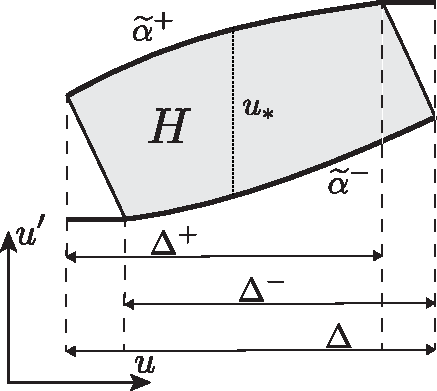
\includegraphics[scale = 1]{pic/thickness definition}
	\caption{An illustration to the definition of an h-strip thickness. Strip $H$ is {\it well-measurable} in a sense of Definition \ref{def:well-measurable-h-strip}. Curves $\widetilde{\alpha}^{\pm}$ are continuations of the initial h-strip borders to the whole $\Delta$; $u_*$ is a point of maximum of the expression \eqref{eq:h-thickness}.}
\label{fig:thickness-definition}
\end{figure}

\begin{proposition}
	For the \emph{h}-strip $H$ the following statement is valid:
	\begin{equation}
		\Delta^+ \cap \Delta^- \neq \varnothing \Rightarrow u_* \in \Delta^+ \cap \Delta^-,
	\end{equation}
	i.e. an \emph{h}-strip is well-measurable if domains of its border functions have at least one common point.
\end{proposition}
\begin{proof}
	Trivially follows from the monotonicity of the h-strip borders $\alpha^+$ and $\alpha^-$.
\end{proof}

In a similar way we define thickness of v-strips.
Let an v-strip $V$ lies inside an island $D$ and is bounded by v-curves $\beta^+$ and $\beta^-$.
Consider this curves as a functions of $u'$: $u = v_{\pm}(u')$.
Denote domains of these functions by $\Delta^{\pm}$.
Continue functions $v_{\pm}(u')$ to the whole interval $\Delta = \Delta^+ \cap \Delta^-$ in the same way as for h-strips, see \eqref{eq:continuation}, and introduce new functions $\widetilde{v}_{\pm}(u')$ and curves $\widetilde{\beta}^{\pm}$.

\begin{definition}
	By the {\bf thickness} of an v-strip $V$, denoted $d_\emph{v}(V)$, we mean the distance between curves $\widetilde{\beta}^{\pm}$ in C-norm, i.e.
	\begin{equation}
		d_\emph{v}(V) = d(\widetilde{\beta}^+, \widetilde{\beta}^-) = \max \limits_{u' \in \Delta} |\widetilde{v}_+(u') - \widetilde{v}_-(u')|.
	\label{eq:v-thickness}
	\end{equation}
\label{def:v-thickness}
\end{definition}

The definition of {\it well-measurable} v-strip is introduced in a same way.
The remark and the proposition above remain valid for the v-strips as well.
Note that thickness of h-strip is measured in a vertical direction, and thickness of v-strip is measured in a horizontal direction.
If a strip is well-measurable then its thickness is measured in a direction along the straight line that connects points from the opposite side of the strip.
This concept will be useful for us during the proof of a theorem about h,v-strips mapping which are formulated in Appendix~\ref{appendix:strips-mapping-theorems}.

\section{Poincar\'e Map Domains for Piecewise Periodic Pseudopotential}

Let's demonstrate how the definitions introduced above work all together.
For that purpose consider a simple form of one-dimensional GPE with periodically modulated pseudopotential
\begin{equation}
	i \Psi_t + \Psi_{xx} + \eta(x) |\Psi|^2 \Psi = 0,
\label{eq:gross-pitaevskii-piecewise}
\end{equation}
where $\eta(x)$ is a periodic piecewise constant function of the period $L = L_* + L_0$:
\begin{equation}
	\eta(x) = \left\{
		\begin{array}{rl}
			-1, & x \in [0; L_*]; \\
			+1, & x \in [L_*; L_* + L_0],
		\end{array}
	\right.
\label{eq:eta}
\end{equation}
\begin{figure}[h]
\centering
	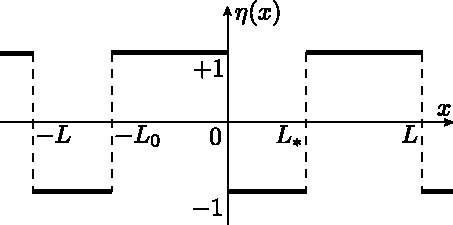
\includegraphics[scale = 1.2]{pic/piecewise constant}
	\caption{\dots}
\label{fig:piecewise-constant}
\end{figure}
This equation is obtained from the initial equation \eqref{eq:gross-pitaevskii} where we put $P(x) = \eta(x)$ and the ordinary potential $U(x)$ is considered to be negligible or even absent, $U(x) \equiv 0$.
Again we consider stationary solutions of the form $\Psi(t, x) = u(x) e^{-i \omega t}, \, \omega \in \mathbb{R}$, where function $u(x)$ satisfies the equation
\begin{equation}
	u_{xx} - \omega u + \eta(x) u^3 = 0. 
\label{eq:stationary-piecewise}
\end{equation}
In order to make things even simpler for our demonstration let's also assume $\omega = 1$.

Since pseudopotential is a piecewise constant function that has only two different values on the period $L$ we can split the period into two regions and consider two different regimes of the equation \eqref{eq:stationary-piecewise}.
In each region the stationary states equation has a familiar form of conservative Duffing equation:
\begin{eqnarray}
	&& u_{xx} - u - u^3 = 0, \quad x \in [0; L_*];\label{eq:stationary-piecewise-singular} \\
	&& u_{xx} - u + u^3 = 0, \quad x \in [L_*; L_* + L_0] \label{eq:stationary-piecewise-regular}.
\end{eqnarray}
Each of the equations \eqref{eq:stationary-piecewise-singular}, \eqref{eq:stationary-piecewise-regular} can be solved explicitly  through Jacobi elliptic functions.
Exact solutions are given in Appendix \ref{appendix-solutions-of-duffing-equations}.
% TODO: Axes size is not consistent with other pictures.
\begin{figure}[h]
\centering
	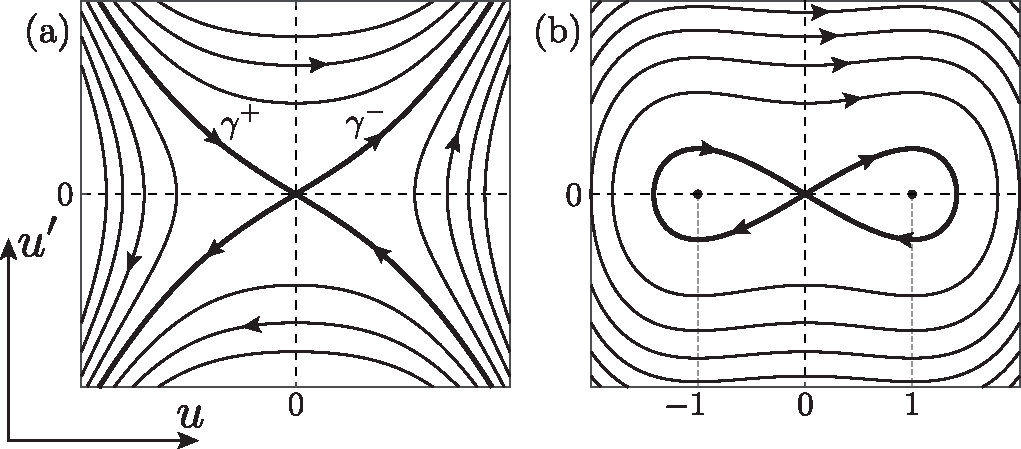
\includegraphics[scale = 1]{pic/phase portraits}
	\caption{Phase portraits for the different regimes of stationary states equation \eqref{eq:stationary-piecewise} with piecewise pseudopotential \eqref{eq:eta}. Panel (a) represents a phase portrait for the equation \eqref{eq:stationary-piecewise-singular}, curves $\gamma^{\pm}$ correspond to the separatrices which enter the equilibrium point $(0, 0)$ as $x$ approaches $\pm \infty$. Panel (b) depicts a phase portrait for the equation \eqref{eq:stationary-piecewise-regular}.}
\label{fig:phase-portraits}
\end{figure}

Equation \eqref{eq:stationary-piecewise-singular} has a first integral of the form:
\begin{equation}
	H_* = u_x^2 - u^2 - \frac{1}{2} u^4.
\label{eq:stationary-piecewise-singular-integral}
\end{equation}
The phase portrait of the equation \eqref{eq:stationary-piecewise-singular} is presented on Figure \ref{fig:phase-portraits} (a).
Any trajectory on the phase plane corresponds to some value of $H_*$.
Level $H_* = 0$ corresponds to the equilibrium state $(0, 0)$, and four separatrices connected to it.
Two of the separatrices $\gamma_{1,2}^+$ enter the zero equilibrium as $x$ approaches $+\infty$.
We denote them along with the point $(0, 0)$ by a curve $\gamma^+$.
Another two separatrices $\gamma_{1,2}^-$ enter the zero equilibrium as $x$ approaches $-\infty$.
Along with the point $(0, 0)$ we denote them by a curve $\gamma^-$ correspondingly.
Result curves $\gamma^{\pm}$ satisfy equations
\begin{equation}
	u' = \pm \frac{u}{\sqrt{2}} \sqrt{2 + u^2}.
\end{equation}

It follows from the exact form of the solutions of the equation \eqref{eq:stationary-piecewise-singular} that all of them, except for the zero one, are singular.
It means that a solution for a Cauchy problem with initial conditions $u(0) = u_0$, $u'(0) = u_0'$ ($u_0$ and $u_0'$ not equals zero simultaneously) tends to infinity while $x$ approaches some finite point both to the left and to the right of $x = 0$.
We say that a solution for the equation \eqref{eq:stationary-piecewise-singular} has a {\it finite domain} if $H_* \neq 0$.
That's why we mark a corresponding period part $L_*$ with a symbol ``$*$'', since the solutions are tend to run out the origin of the phase plane.

The first integral of equation \eqref{eq:stationary-piecewise-regular} is
% TODO: Consider to use (u')^2 instead of (u_x)^2.
\begin{equation}
	H_0 = u_x^2 - u^2 + \frac{1}{2} u^4.
\label{eq:stationary-piecewise-regular-integral}
\end{equation}
Phase portrait for equation \eqref{eq:stationary-piecewise-regular} is given on Figure \ref{fig:phase-portraits} (b).
It has two center equilibrium points $(\pm 1, 0)$ and one hyperbolic equilibrium point $(0, 0)$.
Separatrix loops correspond to the localized solutions
\begin{equation}
	u(x) = \pm \frac{\sqrt{2}}{\cosh{x}}.
\end{equation}
The aria inside the separatrix loops is filled by closed orbits of periodic solutions with nonzero mean.
All other orbits turn around the origin and correspond to solutions with zero mean.
That's why we mark a corresponding period part $L_0$ with a symbol ``$0$'', since it looks like a little curve circle.

\subsection{General Propositions on the $\mathscr{U}_L^{\pm}$ Sets for Piecewise Pseudopotential}

Let's move on to the consideration of the $\mathscr{U}_L^{\pm}$ sets for the equation \eqref{eq:stationary-piecewise}.
Recall that we decided to split the period $L$ into two parts $[0; L_*]$ and $[L_*; L_* + L_0]$.
From that perspective let's consider a decomposition of the Poincar\'e map $\mathcal{P} = \mathcal{P}_0 \mathcal{P}_*$, where  maps associated with corresponding parts of the overall period $L$ are defined in a similar manner as the initial Poincar\'e map $\mathcal{P}$ itself \eqref{eq:poincare-map}.
Map $\mathcal{P}_*$ map a point $(u_0, u_0')$ to $(u(L_*), u'(L_*))$ where $u(x), \, x \in [0; L_*]$ is a solution of Eq.~\eqref{eq:stationary-piecewise-singular} with initial conditions $u(0) = u_0$, $u'(0) = u_0'$.
Similarly map $\mathcal{P}_0$ map a point $(u_0, u_0')$ to $(u(L), u'(L))$ where $u(x), \, x \in [L_*; L]$ is a solution of Eq.~\eqref{eq:stationary-piecewise-regular} with initial conditions $u(L_*) = u_0$, $u'(L_*) = u_0'$.

Note that $\mathcal{P}_*$ cannot be defined everywhere.
We denote by $\mathscr{U}_{L_*}^+$ a domain of the map $\mathcal{P}_*$.
Due to the fact that all solutions of the equation \eqref{eq:stationary-piecewise-regular} are regular, domain of the overall Poincar\'e map $\mathcal{P}$ coincide with the domain of $\mathcal{P}_*$ map, i.e. $\mathscr{U}_L^+ = \mathscr{U}_{L_*}^+$.
For the equation \eqref{eq:stationary-piecewise} it can be written as follows:
\begin{equation}
	\mathscr{U}_L^+ = \textrm{dom}(\mathcal{P}) = \textrm{dom}(\mathcal{P}_0 \mathcal{P}_*) = \textrm{dom}(\mathcal{P}_*) \equiv \mathscr{U}_{L_*}^+.
\end{equation}

It's easy to note several other properties of the $\mathscr{U}_{L_*}^+$ set.
Since the phase portrait for Eq.~\eqref{eq:stationary-piecewise-singular} is symmetric with respect to the origin, $\mathscr{U}_{L_*}^+$ is also symmetric with respect to the origin.
Two separatrices that correspond to the curve $\gamma^+$ are tend to zero equilibrium as $x \to +\infty$.
It means that for any initial data posed at $\gamma^+$ and for any $L_*$ the map $\mathcal{P}_*$ is correctly defined, i.e. $\gamma^+ \in \mathscr{U}_{L_*}^+$.
Another property of $\mathscr{U}_{L_*}^+$ directly follows from Proposition \ref{prop:domain-reflection}:
\begin{equation}
	\mathcal{P}_*(\mathscr{U}_{L_*}^+) = I (\mathscr{U}_{L_*}^+) = \mathscr{U}_{L_*}^-.
\label{eq:domain-reflection-singular-forward}
\end{equation}
% TODO: A comprehensive theorem can be added here.
%   1. Borders of $\mathscr{U}_{L_*}^+$ are decreasing curves.
%   2. Distance between borders tends to zero as $u \to \infty$, $u' \to \infty$.

Move on to the $\mathscr{U}_{L_*}^-$ set for equation \eqref{eq:stationary-piecewise-singular}.
Since $\mathscr{U}_{L_*}^-$ is a reflection of $\mathscr{U}_{L_*}^+$ set with respect to the $u'$ axis, it inherits its symmetry properties.
Set $\mathscr{U}_{L_*}^-$ also contains curve $\gamma^-$ that corresponds to another two separatrices $\gamma_{1,2}^-$ of equation \eqref{eq:stationary-piecewise-singular}.
% TODO: A comprehensive theorem can be added here.
%   1. Borders of $\mathscr{U}_{L_*}^-$ are decreasing curves.
%   2. Distance between borders tends to zero as $u \to \infty$, $u' \to \infty$.
Consider the second map $\mathcal{P}_0$ of the decomposition.
As we mentioned above $\mathcal{P}_0$ correctly defined on the whole $\mathscr{U}_{L_*}^-$.
If so, it's interesting to figure out how this map transform separatrices curve $\gamma^-$.
It turns out that the image $\mathcal{P}_0(\gamma^-)$ has a spiral-like structure and intersects the curve $\gamma^+$ infinitely many times.
The following proposition can be proved.

% TODO: Consider to use `tfrac`.
% TODO: Consider to use $\mathcal{O}(n^{-1})$ instead of $\mathcal{O}(H^{\nicefrac{-1}{4}})$.
\begin{proposition}
	$\mathcal{P}_0$-image of the curve $\gamma^-$ intersects $\gamma^+$ infinitely many times at the points $\{ 0 \} \cup {u_{\pm n}}$,
	\begin{equation}
		u_{\pm n} = \pm \frac{2 x_{n-1}}{\sqrt[4]{2} L_0} + \mathcal{O} \left( H_0^{\nicefrac{-1}{4}} \right), \ n \in \mathbb{N},
	\label{eq:separatrix-map-un}
	\end{equation}
	as $H_0 \to \infty$, $x_n$ are determined as
	\begin{equation}
		x_n = \cn^{-1} \left( 2^{\nicefrac{-1}{4}}, k_0 \right) + K(k_0) n,
	\label{eq:separatrix-map-xn}
	\end{equation}
	where $K(k)$ is the complete elliptic integral of the first kind, and $k_0 = 1 / \sqrt{2}$. 
\label{prop:separatrix-map}
\end{proposition}
\begin{proof}
	First of all, point $(0, 0)$ belongs to the intersection $\mathcal{P}_0(\gamma^-) \cap \gamma^+$ since it's a stable fixed point of equation \eqref{eq:stationary-piecewise-regular} and the $\mathcal{P}_0$ map.

	Next we note that all the intersections $\mathcal{P}_0(\gamma^-) \cap \gamma^+$ occur outside of the separatrix loops of \eqref{eq:stationary-piecewise-regular} and correspond to zero mean solutions of \eqref{eq:stationary-piecewise-regular}.
	This obviously follows from that fact that $\gamma^+$ lies outside of the loops both from left and right of $u'$ axis (depicted on Fig.~\ref{fig:separatrix-map}~(a)).
	\begin{figure}[h]
	\centering
		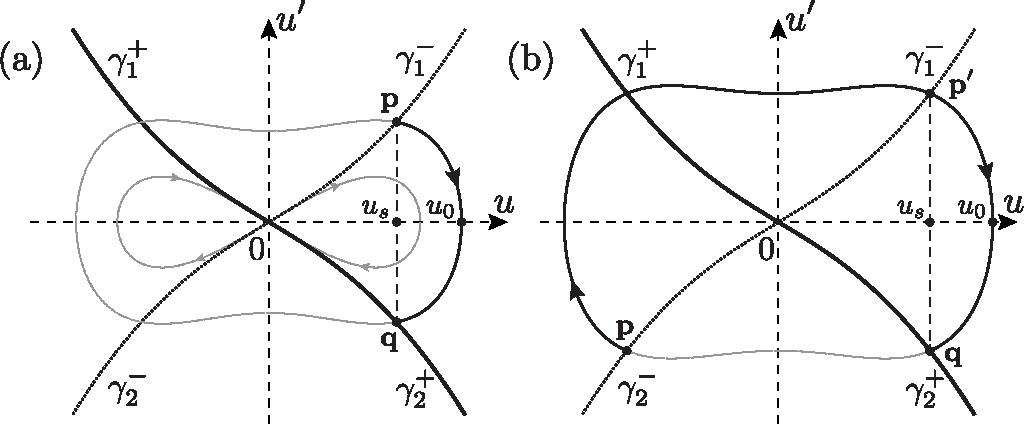
\includegraphics[scale = 1]{pic/separatrix map}
		\caption{Illustration for the proof of Proposition~\ref{prop:separatrix-map}.}
	\label{fig:separatrix-map}
	\end{figure}
	
	Prove the formula for points from the right side of $u'$ axis, $u_{+n}$.
	Such points corresponds to the $\gamma_2^+$ separatrix of equation \eqref{eq:stationary-piecewise-singular}, see Figure~\ref{fig:separatrix-map}.
	Result points of intersections $\mathcal{P}_0(\gamma^-) \cap \gamma_2^+$ can be divided into two groups: $\mathcal{P}_0(\gamma_1^-) \cap \gamma_2^+$ and $\mathcal{P}_0(\gamma_2^-) \cap \gamma_2^+$.

	Consider points from the first group.
	Let a point $\vb{q}$ belongs to the intersection $\mathcal{P}_0(\gamma_1^-) \cap \gamma_2^+$.
	Then there exists a point $\vb{p} = (u_s, u_s') \in \gamma_1^-$ such that $\mathcal{P}_0(\vb{p}) \in \gamma_2^+$.
	Due to the symmetries of the phase portraits for equations \eqref{eq:stationary-piecewise-singular} and \eqref{eq:stationary-piecewise-regular}, $\vb{q} = (u_s, -u_s')$, see Figure~\ref{fig:separatrix-map}~(a).
	Consider a phase trajectory of \eqref{eq:stationary-piecewise-regular} that lies outside of separatrix loop and connects points $\vb{p}$ and $\vb{q}$.
	According to Appendix~\ref{appendix:solutions-of-duffing-equations} exact form of the solution is
	\begin{equation}
		u(x) = x_0 \cn \left( \sqrt{x_0^2 - 1} x + x_1, k \right),
	\label{eq:stationary-piecewise-regular-solution}
	\end{equation}
	where $k$ is elliptic modulus, $k = \dfrac{1}{\sqrt{2}} \dfrac{x_0}{\sqrt{x_0^2 - 1}}$, and $x_0$, $x_1$ are constants that can be determined by initial conditions $(u(0), u'(0)) = \vb{p}$.
	
	Next let's introduce an $x$ variable shift $x \to x - L_0 / 2$.
	Equation \eqref{eq:stationary-piecewise-regular-solution} persists its form but now $u(0) = u_0, \ u_0 > 0$, and $u'(0) = 0$.
	That allows us to determine constants $x_0, \, x_1$: $x_0 = u_0,$ $x_1 = 0$.
	Solution \eqref{eq:stationary-piecewise-regular-solution} takes form
	\begin{equation}
		u(x) = u_0 \cn \left( \sqrt{u_0^2 - 1} x, k \right),
	\label{eq:stationary-piecewise-regular-solution-shifted}
	\end{equation}
	and for coordinates of the points $\vb{p}$ and $\vb{q}$ we have
	\begin{alignat}{3}
		& \vb{p} = (u(-L_0 / 2), && \ u'(-L_0 / 2)) && = (u_s, u_s'); \label{eq:p-first-group} \\
		& \vb{q} = (u(L_0 / 2),  && \ u'(L_0 / 2)) && = (u_s, -u_s'). \label{eq:q-first-group}
    \end{alignat}
	Now we use the fact that value of $H_0$ \eqref{eq:stationary-piecewise-regular-integral} remains the same along the trajectory that connects point $\vb{p}$ and the point $(u_0, 0)$ of intersection between trajectory and the $u$ axis.
	Thus one can write the following relationship:
	\begin{equation}
		H_0 = -u_0^2 + \frac{u_0^4}{2} = (u_s')^2 - u_s^2 + \frac{u_s^4}{2}.
	\label{eq:trajectory-H0}
	\end{equation}
	On the other hand point $\vb{p}$ belong to the separatrix of \eqref{eq:stationary-piecewise-singular} and its coordinates satisfy an equality
	\begin{equation}
		H_* = (u_s')^2 - u_s^2 - \frac{u_s^4}{2} = 0.
	\label{eq:separatrix-H*}
	\end{equation}
	Comparing \eqref{eq:trajectory-H0} and \eqref{eq:separatrix-H*} one can conclude
	\begin{equation}
		u_s^4 = \frac{u_0^4}{2} - u_0^2.
	\label{eq:separatrix-u-coordinate}
	\end{equation}
	The next step is to consider equation \eqref{eq:stationary-piecewise-regular-solution} at the point $\vb{q}$, we have
	\begin{equation}
		u_s = u_0 \cn \left(\frac{\sqrt{u_0^2 - 1} L_0}{2}, k \right).
	\label{eq:stationary-piecewise-regular-solution-q}
	\end{equation}
	Put $u_s$ from \eqref{eq:separatrix-u-coordinate} into \eqref{eq:stationary-piecewise-regular-solution-q}, divide both side of the equality by $u_0$, and introduce a variable change $4 v_0^2 = u_0^2 - 1$.
	Equation \eqref{eq:stationary-piecewise-regular-solution-q} takes form
	\begin{equation}
		\left( \frac{1}{2} - \frac{1}{4 v_0^2 + 1} \right)^{1/4} = \cn \left( v_0 L_0, k \right), \quad k = \frac{1}{\sqrt{2}} \sqrt{1 + \frac{1}{4 v_0^2}}.
	\label{eq:v0-elliptic-relationship}
	\end{equation}
	
	In order to get final the result we need to simplify the expression \eqref{eq:v0-elliptic-relationship}.
	First of all consider $k$ as a function of $v_0$ and expand it into a series:
	\begin{equation}
		k(v_0) = \frac{1}{\sqrt{2}} + \frac{1}{8 \sqrt{2}} \frac{1}{v_0^2} - \frac{1}{32 \sqrt{2}} \frac{1}{v_0^4} + \dots.
	\label{eq:k-series}
	\end{equation}
	Let $k_0 = 1/\sqrt{2}$ and introduce a remainder $\Delta k = k(v_0) - k_0$.
	We keep in mind that $\Delta k$ has a main term of order $v_0^{-2}$ as $v_0 \to \infty$.
	Denote $w_0 = v_0 L_0$, consider $\cn(w_0, k)$ in the right side of \eqref{eq:v0-elliptic-relationship} as a function of elliptic modulus $k$ and expand it into a series in the vicinity of $k_0$ up to the second term:
	\begin{equation}
		\cn \left( w_0, k_0 + \Delta k \right) = \cn \left( w_0, k_0 \right) + f(w_0, k_0) \Delta k + \mathcal{O}(w_0^{-1/4}).
	\label{eq:elliptic-cosine-expansion}
	\end{equation}
	Here $f(w_0, k_0)$ is the first derivative of elliptic cosine with respect to $k$ at $k = k_0$:
	% TODO: Give a link to Abramowitz and Stegun.
	\begin{equation}
		f(w_0, k_0) = \frac{\sn (w_0) \dn (w_0) (w_0 - k_0 w_0 + k_0 \sn(w_0) \cd(w_0) - E(\phi(w_0))) }{2 (k_0 - 1) k_0} .
	\end{equation}
	Here $\phi(w, k)$ is the Jacobi amplitude and $E(\phi, k)$ is the incomplete elliptic integral of the second kind.
	All elliptic functions have the same modulus $k_0$, we omit this parameter for the sake of brevity.
	This expression is quite tremendous, nevertheless, what interests us here is the orders of terms with respect to $w_0$.
	It has a leading term of order $w_0$ as $w_0 \to \infty$.
	That allows us to conclude that the term $f(w_0, k_0) \Delta k$ of \eqref{eq:elliptic-cosine-expansion} in its turn has a leading term of order $w_0^{-1}$ (or $v_0^{-1}$).
	Rewrite relationship \eqref{eq:v0-elliptic-relationship} in a new form:
	\begin{equation}
		\left( \frac{1}{2} - \frac{1}{4 v_0^2 + 1} \right)^{1/4} = \cn \left( v_0 L_0, k_0 \right) + \mathcal{O}(v_0^{-1}),
	\label{eq:v0-elliptic-relationship-asymptotic}
	\end{equation}
	Using the same approach again we expand the left side of \eqref{eq:v0-elliptic-relationship-asymptotic} into a series:
	\begin{equation}
		\left( \frac{1}{2} - \frac{1}{4 v_0^2 + 1} \right)^{1/4} =  \frac{1}{\sqrt[4]{2}} - \frac{1}{2 \sqrt[4]{2}} \frac{1}{(4v_0^2 + 1)} + \mathcal{O}(v_0^{-4}).
	\label{eq:v0-elliptic-relationship-left-side-expansion}
	\end{equation}
	Combining \eqref{eq:v0-elliptic-relationship-left-side-expansion} with \eqref{eq:v0-elliptic-relationship-asymptotic} and comparing the orders of terms we conclude that
	\begin{equation}
		\cn (v_0 L_0, k_0) = \frac{1}{\sqrt[4]{2}} + \mathcal{O}(v_0^{-1}).
	\end{equation}
	Let's express $v_0 L_0$ in the equation above 
	\begin{equation}
		v_0 L_0 = \cn^{-1} \left( \frac{1}{\sqrt[4]{2}} + \mathcal{O}(v_0^{-1}), k_0 \right) + 2 K(k_0) n, \quad n \in \{0\} \cup \mathbb{N}.
	\label{eq:v0-L0-expression}
	\end{equation}
	Here $K(k)$ is the complete elliptic integral of the first kind. 
	We left only positive roots since we are interested only in intersections $\mathcal{P}_0(\gamma_1^-) \cap \gamma_2^+$ where $u_0$ is positive and we can write
	\begin{equation}
		v_0 = \frac{u_0}{2} \sqrt{1 - \frac{1}{u_0^2}} = \frac{u_0}{2} - \frac{1}{2u_0} + \mathcal{O}(u_0^{-3}).
	\label{eq:v0-through-u0}
	\end{equation}
	We note that by definition of $\cn^{-1}$ function
	\begin{equation}
		\cn^{-1} \left( 2^{\nicefrac{-1}{4}} + \mathcal{O}(v_0^{-1}) \right) = F \left( \arccos \left( 2^{\nicefrac{-1}{4}} + \mathcal{O}(v_0^{-1}) \right), k_0 \right),
	\label{eq:inverse-elliptic-cosine-definition}
	\end{equation}
	where $F(\phi, k)$ is incomplete elliptic integral of the first kind.
	Consider series expansion of $\arccos$ up to the main term:
	\begin{equation}
		\arccos \left( 2^{\nicefrac{-1}{4}} + \mathcal{O}(v_0^{-1}) \right) = \arccos \left( 2^{\nicefrac{-1}{4}} \right) + \mathcal{O}(v_0^{-1}).
	\label{eq:arccos-expansion}
	\end{equation}
	Let's substitute \eqref{eq:arccos-expansion} into \eqref{eq:inverse-elliptic-cosine-definition}, use additive property of integral, and apply integral mean value theorem to the second term:
	\begin{equation}
	\begin{split}
		\cn^{-1} \left( 2^{\nicefrac{-1}{4}} + \mathcal{O}(v_0^{-1}) \right) & = F \left( \arccos \left( 2^{\nicefrac{-1}{4}} \right) + \mathcal{O}(v_0^{-1}), k_0 \right) = \\ & = F \left( \arccos \left( 2^{\nicefrac{-1}{4}} \right), k_0 \right) + F \left( \mathcal{O}(v_0^{-1}), k_0 \right) = \\ & = \cn^{-1} \left( 2^{\nicefrac{-1}{4}}, k_0 \right) + \mathcal{O}(v_0^{-1}).
	\end{split}
	\label{eq:inverse-elliptic-cosine-asymptotic}
	\end{equation}
	Put \eqref{eq:inverse-elliptic-cosine-asymptotic} and \eqref{eq:v0-through-u0} into \eqref{eq:v0-L0-expression}, also note that according to \eqref{eq:v0-through-u0} we can safely replace $\mathcal{O}(v_0^{-1})$ with $\mathcal{O}(u_0^{-1})$,
	\begin{equation}
		u_0 = \frac{2}{L_0} \left( \cn^{-1} \left( 2^{\nicefrac{-1}{4}}, k_0 \right) + 2 K(k_0) n \right) + \mathcal{O}(u_0^{-1}).
	\label{eq:u0-expression}
	\end{equation}
	Finally let's get rid of $u_0$ in favor of $u_s$.
	For that purpose according to \eqref{eq:trajectory-H0} we can write $\mathcal{O}\left(H_0^{\nicefrac{-1}{4}}\right)$ instead of $\mathcal{O}(u_0^{-1})$, and it follows from \eqref{eq:separatrix-u-coordinate} that
	\begin{equation}
		u_s = \dfrac{1}{\sqrt[4]{2}} u_0 + \mathcal{O}(u_0^{-1}).	
	\end{equation}
	Let's introduce the following denotation
	\begin{equation}
		x_n = \cn^{-1} \left( 2^{\nicefrac{-1}{4}}, k_0 \right) + 2K(k_0)n.
	\label{eq:xn-first-group}
	\end{equation}
	Now combining the expressions above all together and replacing $u_s$ with $u_{+n}$ we get
	\begin{equation}
		u_{+n} = \frac{2 x_{n-1}}{\sqrt[4]{2} L_0} + \mathcal{O} \left( H_0^{\nicefrac{-1}{4}} \right), \quad n \in \mathbb{N}.
	\label{eq:un-final-positive}
	\end{equation}
	
	In order to get the final formula of the proposition for $\{ u_{+n} \}$ we need to consider points of intersections from the second group $\mathcal{P}_0 (\gamma_2^-) \cap \gamma_2^+$.
	We can easily reduce this task to the previous one.
	Let there exists a point of intersection $\vb{q} \in \gamma_2^+$. 
	Consider point $\vb{p} \in \gamma_2^-$, such that $\mathcal{P}_0(\vb{p}) = \vb{q}$, see Fig.~\ref{fig:separatrix-map}~(b).
	We note that there exists a point $\vb{p}' \in \gamma_1^-$, and the trajectory \eqref{eq:stationary-piecewise-regular-solution} goes from the point $\vb{p}$ to $\vb{p}'$ over a half of the period $2K(k) / \sqrt{x_0^2 - 1}$, and after that cross the $u$ axis at the point $u_0$.
	Then we introduce an $x$ variable shift $x \to x - (L_0 / 2 + K(k) / \sqrt{x_0^2 - 1})$, so that $u(0) = u_0, \ u_0 > 0$, and $u'(0) = 0$, and can determine $x_0 = u_0$, $x_1 = 0$.
	Solution \eqref{eq:stationary-piecewise-regular-solution} takes form \eqref{eq:stationary-piecewise-regular-solution-shifted} again and for coordinates of the points $\vb{p}'$ and $\vb{q}$ we have
	\begin{alignat}{4}
		& \vb{p}' && = \bigg( u \bigg( -L_0 / 2 + \tfrac{K(k)}{\sqrt{u_0^2 - 1}} \bigg), && \ u' \bigg( -L_0 / 2 + \tfrac{K(k)}{\sqrt{u_0^2 - 1}} \bigg) \bigg) && = (u_s, u_s'); \label{eq:p'-second-group} \\
		& \vb{q} && = \bigg( u \bigg(L_0 / 2 - \tfrac{K(k)}{\sqrt{u_0^2 - 1}} \bigg),  && \ u' \bigg( L_0 / 2 - \tfrac{K(k)}{\sqrt{u_0^2 - 1}} \bigg) \bigg) && = (u_s, -u_s'). \label{eq:q-second-group}
    \end{alignat}
    Now we can use relationships \eqref{eq:p'-second-group}, \eqref{eq:q-second-group} instead of \eqref{eq:p-first-group}, \eqref{eq:q-first-group}, and repeat all the steps above.
    Difference in $x$ variable shift results in the additional term $K(k)$ in \eqref{eq:v0-L0-expression} and \eqref{eq:u0-expression}.
    Finally we replace $K(k) = K(k_0 + \Delta k) = K(k_0) + \mathcal{O}(H_0^{\nicefrac{-2}{4}})$, and get the following relationship for $x_n$:
	\begin{equation}
		x_n = \cn^{-1} \left( 2^{\nicefrac{-1}{4}}, k_0 \right) + K(k_0) (2n + 1).
	\label{eq:xn-second-group}
	\end{equation}
	Relationship \eqref{eq:un-final-positive} remains the same.
	Combining \eqref{eq:xn-first-group} with \eqref{eq:xn-second-group} we get the result for separatrix intersections points $\{ u_{+n} \} \in \mathcal{P}(\gamma^-) \cap \gamma_2^+$:
	\begin{equation}
		u_{+n} = \frac{2 x_{n-1}}{\sqrt[4]{2} L_0} + \mathcal{O} \left( H_0^{\nicefrac{-1}{4}} \right), \quad n \in \mathbb{N},
	\label{eq:us-final}
	\end{equation}
	where $x_n$ satisfies the relationship
	\begin{equation}
		x_n = \cn^{-1} \left( 2^{\nicefrac{-1}{4}}, k_0 \right) + K(k_0) n.
	\label{eq:xn-final}
	\end{equation}
	
	Points $\{ u_{-n} \} , \ n \in \mathbb{N}$ from the left side of $u'$ axis, $u_{-n} \in \mathcal{P}_0(\gamma^-) \cap \gamma_1^+$, should be treated in a similar way, proposition is proven.
\end{proof}

Propositions~\ref{prop:separatrix-map} says that the far we goes from the $(0, 0)$ point on the phase plane, the better the asymptotic relationship \eqref{eq:separatrix-map-un} works.
It turns out that formula \eqref{eq:separatrix-map-un} works pretty well even for small number of $n$.
See Figure~\ref{fig:separatrix-map-with-numerical-computations} where we compare the predicted coordinates with actual intersections obtained by numerical computation of $\mathcal{P}_0(\gamma^-)$.
Another interesting consequence of Proposition~\ref{prop:separatrix-map} is that set $\mathscr{U}_{L}$ consists of infinitely many connected components.
This obviously follows from that fact, that set $\mathscr{U}_{L_*}^-$ contains the entire curve $\gamma^-$ and map $\mathcal{P}_0$ is continuous, so the image $\mathcal{P}_0 (\mathscr{U}_{L_*}^-)$ cross $\mathscr{U}_{L}^+$ infinitely many times.
\begin{figure}[h]
\centering
	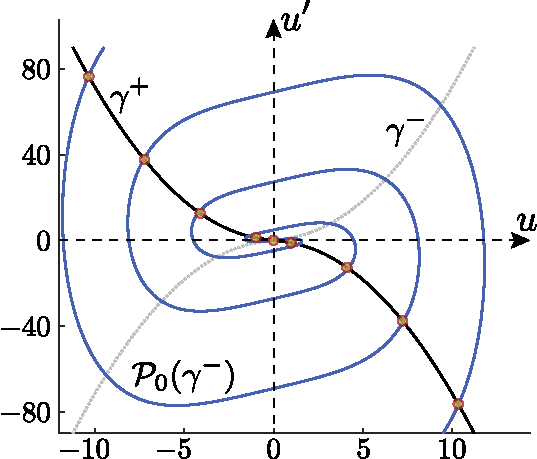
\includegraphics[scale = 1]{pic/separatrix map with numerical computations}
	\caption{
		Comparison of the relationship \eqref{eq:separatrix-map-un} from Proposition~\ref{prop:separatrix-map} with numerical computations.
		Curves $\gamma^{\pm}$ are formed by the separatrices of \eqref{eq:stationary-piecewise-singular}, $\mathcal{P}_0$-image of $\gamma^-$ is a solid blue line computed numerically.
		Predicted points of intersections $u_{\pm n}$ from $\mathcal{P}_0(\gamma^-) \cap \gamma^+$ are marked with yellow dots. One can see that \eqref{eq:separatrix-map-un} predicts intersections quite precisely even for small number of $n$.
	}
\label{fig:separatrix-map-with-numerical-computations}
\end{figure}

\subsection{Construction of the Poincar\'e Map Domains}

One of the possible way to construct $\mathscr{U}_L^{\pm}$ sets for different maps associated with stationary states equation \eqref{eq:stationary} is to use a numerical procedure called scanning of initial conditions plane $(u, u')$.
That's how it works.
At first ranges of scanning $u_{\min} \le u \le u_{\max}$, $u_{\min}' \le u' \le u_{\max}'$ are selected.
Then the target segment of the initial conditions plane is covered by a uniform grid with small steps $h$ and $h'$ for each axis $u$ and $u'$.
Using Runge-Kutta 4th order method we solve differential equation in each node of the result grid.
We use an interval $[0; L]$ for $\mathscr{U}_L^+$ where $x$ changes in forward direction from $0$ to $L$, and an interval $[-L; 0]$ in order to get $\mathscr{U}_L^-$ where $x$ changes in backward direction from $0$ to $-L$.
If absolute value of a calculated solution does not exceed some huge predefined constant $M$ we suppose that such solution is non-collapsing, and include corresponding node point into $\mathscr{U}_L^{\pm}$ sets.
Then we color non-collapsing nodes on the initial conditions plane to get the final picture of $\mathscr{U}_L^{\pm}$ sets.
In our experiments we used $M = 10^5$ and $M = 10^7$, and got consistent results.
Such procedure is pretty straightforward and can be efficiently performed by a computer since it admits natural parallelization.
Let's apply this procedure to equation \eqref{eq:stationary-piecewise}.

\begin{figure}[h]
\centering
	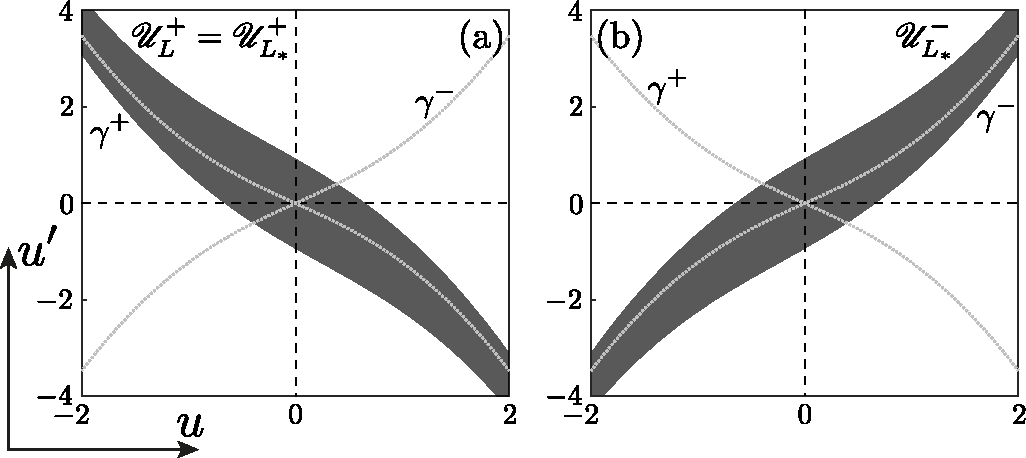
\includegraphics[scale = 1]{pic/Poincare map domain for piecewise singular equation}
	\caption{
		Sets $\mathscr{U}_{L_*}^{\pm}$ for the equation \eqref{eq:stationary-piecewise-singular} for the parameter $L_* = 2$.
		Panel (a) represents $\mathscr{U}_{L_*}^+$ set, it coincides with the set $\mathscr{U}_L^+$ for equation \eqref{eq:stationary-piecewise}, since all solutions of the second equation \eqref{eq:stationary-piecewise-regular} are regular.
		Panel (b) depicts $\mathscr{U}_{L_*}^-$ set, it's just a reflection of the set $\mathscr{U}_L^+$ from the right panel due to Proposition~\ref{prop:domain-reflection}.
	}
\label{fig:poincare-map-domain-piecewise}
\end{figure}

On Figure~\ref{fig:poincare-map-domain-piecewise}~(a) Poincar\'e map   domain $\mathscr{U}_L^+ = \mathscr{U}_{L_*}^+$ for the parameters $(L_*, L_0) = (2, 1)$ is depicted.
As we mentioned above it contains the curve $\gamma^+$ formed by separatrices of \eqref{eq:stationary-piecewise-singular}.
Figure~\ref{fig:poincare-map-domain-piecewise}~(b) represents a $\mathcal{P}_*$-image of $\mathscr{U}_{L_*}^+$, $\mathcal{P}_* (\mathscr{U}_{L_*}^+) = \mathscr{U}_{L_*}^-$.
According to Proposition~\ref{prop:domain-reflection} set $\mathcal{P}_*(\mathscr{U}_{L_*}^-)$ can be obtained by a reflection of the set $\mathscr{U}_{L_*}^+$, with respect to the $u'$ axis.
Set $\mathscr{U}_{L_*}^-$ in its turn contains curve $\gamma^-$.

Let's continue our scanning in order to get set $\mathscr{U}_L^-$ and then intersect it with $\mathscr{U}_L^+$.
On Figure~\ref{fig:island-set-piecewise}~(a) set $\mathscr{U}_L^-$ and its intersection with $\mathscr{U}_L^+$ set are depicted for values of parameters $(L_*, L_0) = (2, 1)$.
From our numerical procedure we can conclude that intersection $\mathscr{U}_L = \mathscr{U}_L^+ \cap \mathscr{U}_L^-$ form a three-island set in the scanning area $-2 \le u \le 2$, $-4 \le u' \le 4$, denote them by $D_i, \, i \in \{ -1, 0, +1 \}$.
Indeed, along with the monotonicity of the connected components borders we also know that two opposite borders of $D_i$, which entirely belong to the borders of the set $\mathscr{U}_L^+$, consist of points that are mapped to infinity under action of $\mathcal{P}$ (by construction of $\mathscr{U}_L^+$).
On other hand borders of $\mathscr{U}_L^-$ contain two other borders of each $D_i$, and they are mapped to infinity under action of $\mathcal{P}^{-1}$.
Thereby the obtained structure satisfy all the conditions of island set from Definition~\ref{def:island-set}.
However set $\mathscr{U}_L^-$ entirely contains an image of the curve $\gamma^-$.
We know that according to Proposition~\ref{prop:separatrix-map} image $\mathcal{P}(\gamma^-)$ has infinitely many intersections with the curve $\gamma^+$.
That's why outside of the scanning area there exist many other intersections between $\mathscr{U}_L^{\pm}$ sets and they form infinitely many connected components in the result set $\mathscr{U}_L$.
Due to monotonicity of $\mathscr{U}_L^+$ borders and general geometric properties of the spiral $\mathscr{U}_L^-$ we can hypothesize that all other intersections in $\mathscr{U}_L$ set are also islands.

% TODO: Add image of $\gamma^-$ to the pictures.
\begin{figure}[h]
\centering
	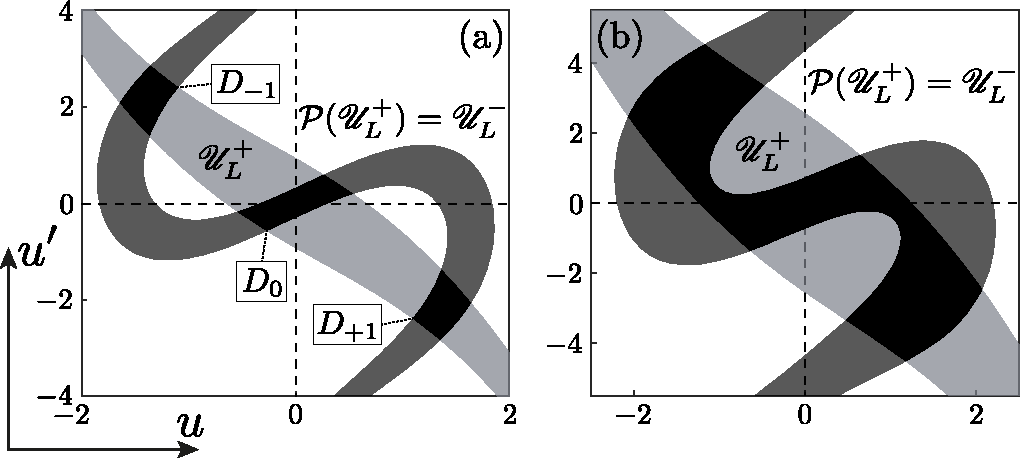
\includegraphics[scale = 1]{pic/island set for piecewise equation}
	\caption{
		Sets $\mathscr{U}_L^+$ (light gray), $\mathscr{U}_L^-$ (dark gray), and their intersection $\mathscr{U}_L$ for two different sets of parameters.
		Panel (a) depict the case $(L_*, L_0) = (2, 1)$; three central connected components $D_i$ form an island set.
		Panel (b) correspond to the case $(L_*, L_0) = (1.3, 1)$; geometry of the result sets does not allow to form islands.
	}
\label{fig:island-set-piecewise}
\end{figure}

Our numerical studies shows that for equation \eqref{eq:stationary-piecewise} three central components of $\mathscr{U}_L$ play a crucial role in an island set formation.
For example on Figure~\ref{fig:islands-set}~(b) geometry of the $\mathscr{U}_L^-$ for parameters $(L_*, L_0) = (1.3, 1)$ does not allow to form an island around the center.
% TODO: Give links to works of Alfimov and Kizin where island set has been studied in details.
Establishing a criteria of island set existence is a quite tricky task even for a simple form of stationary states equation with periodic pseudopotential $P(x)$, like \eqref{eq:stationary-piecewise}, and such criteria is out of scope for the current work.
Our approach here and after is based on scanning of a sufficiently large subset of initial conditions plane around the center $(u, u') = (0, 0)$.
If the result subset of $\mathscr{U}_L$ form an island set we just {\it make a hypothesis} that all other intersections and also islands.

\subsection{Complete Islands Set}

Let $\mathscr{U}_L$ represents an island set.
It turns out that for Eq.~\eqref{eq:stationary-piecewise} the property of ``completeness''  for an island set in a sense of Definition~\ref{def:complete-island-set} naturally arises from its construction.
Let's demonstrate it in a non-strict manner.
At first, upper boundary of the set $\mathscr{U}_L^+ = \mathscr{U}_{L_*}^+$ consist of such points that the corresponding solution to the Cauchy problem with initial conditions at these points tends to $+\infty$ exactly at the point $x = L_*$.
This can be easily followed from the phase portrait for equation \eqref{eq:stationary-piecewise-singular}.
We can say that such points are mapped to $(+\infty, +\infty)$ under action of $\mathcal{P}_*$, i.e. are mapped to infinity toward the right upper corner on the phase plane.
From that perspective lower boundary of the set $\mathscr{U}_L^+$ consists of points that are mapped to $(-\infty, -\infty)$ by $\mathcal{P}_*$, i.e. are mapped to infinity toward the left lower corner on the phase plane.

Let's consider a curve $\Gamma$ inside one of islands $D_i \in \mathscr{U}_L$ that connects opposite boundaries of the set $\mathscr{U}_L^+$.
Denote by $\Gamma_*$ its $\mathcal{P}_*$-image, $\Gamma_* = \mathcal{P}_*(\Gamma)$.
It's clear that $\Gamma_*$ belongs to $\mathscr{U}_{L_*}^-$, and it's stretched out continuously from $-\infty$ to $+\infty$ by $u$ inside $\mathscr{U}_{L_*}^-$.
Now consider the second map $\mathcal{P}_0$ of the decomposition $\mathcal{P} = \mathcal{P}_0 \mathcal{P}_*$.
We know that this map curls the set $\mathscr{U}_{L_*}^-$ into a spiral (see Fig.~\ref{fig:island-set-piecewise}~(a)).
This spiral intersects $\mathscr{U}_L^+$ and form islands.
So if we consider the $\mathcal{P}_0$-image of $\Gamma_*$ and take into account that the value of $H_0$ remains the same for all trajectories of \eqref{eq:stationary-piecewise-regular} associated with $\mathcal{P}_0$ map, we can conclude that $\mathcal{P}_0(\Gamma_*)$ is stretched along the whole set $\mathscr{U}_L^-$ and intersects each of the islands $D_i \in \mathscr{U}_L$ at least once.
Such reasoning leads us to the conclusion that all islands in $\mathscr{U}_L$ are forward-reachable.
Similar consideration shows that islands from $\mathscr{U}_L$ are also backward-reachable and the constructed island set is complete.

Let's illustrate this idea.
For that purpose we construct $\mathcal{P}_*$ and $\mathcal{P}$-images of islands from Figure~\ref{fig:island-set-piecewise}~(a).
Again we do this numerically with the scanning procedure described above.
On Figure~\ref{fig:map-of-islands-piecewise}~(a) one can see the $\mathcal{P}_*$-image of islands $D_i$, $i \in \{ -1, 0, +1\}$.
As we have expected these images represent infinite curvilinear strips stretched inside the $\mathcal{P}_*$-image of the $\mathscr{U}_L^+$ set.
Islands $\mathcal{P}$-images depicted on Figure~\ref{fig:map-of-islands-piecewise}~(b).
Images $\mathcal{P}(D_i)$ represents infinite curvilinear strips curled up inside the $\mathscr{U}_L^-$ set.

\begin{figure}[h]
\centering
	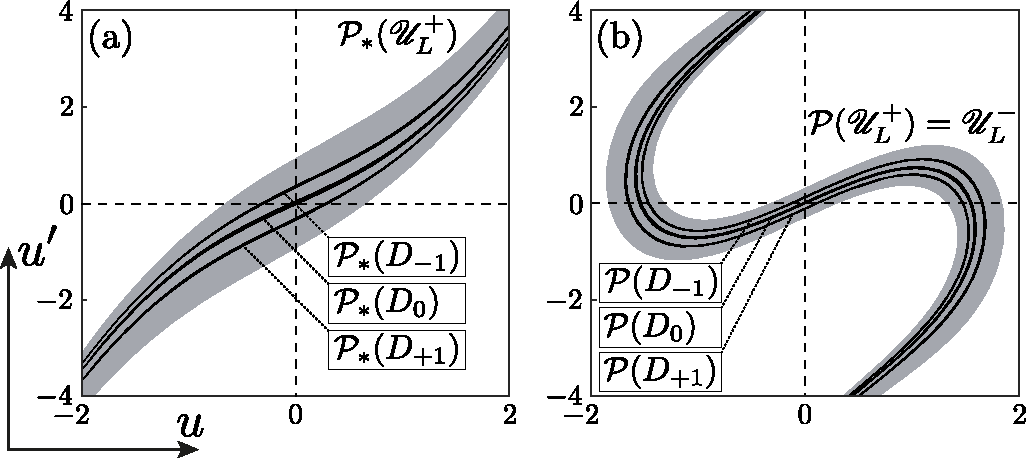
\includegraphics[scale = 1]{pic/Poincare map of islands for piecewise equation}
	\caption{
		$\mathcal{P}_*$ and $\mathcal{P}$-images of islands formed for Eq.~\eqref{eq:stationary-piecewise} for parameters $(L_*, L_0) = (2, 1)$.
		Panel (a) represents their $\mathcal{P}_*$-images.
		Each image is a curvilinear strip stretched along the whole $\mathcal{P}_*(\mathscr{U}_L^+)$.
		Panel (b) represents $\mathcal{P}$-images.
	}
\label{fig:map-of-islands-piecewise}
\end{figure}

Images $\mathcal{P}(D_i)$ remind the behaviour of the separatrices curve image $\mathcal{P}_0(\gamma^-)$.
Each of them intersects the $\mathscr{U}_L^+$ set infinitely many times and cross each island from $\mathscr{U}_L$.
To illustrate that on Figure~\ref{fig:h-strips-piecewise} we combined Figure~\ref{fig:map-of-islands-piecewise}~(b) with Figure~\ref{fig:island-set-piecewise}~(a).
We use the following notation $\mathcal{P}(D_i) \cap D_j = H_{ij}$.

\pagebreak

\begin{figure}[h]
\centering
	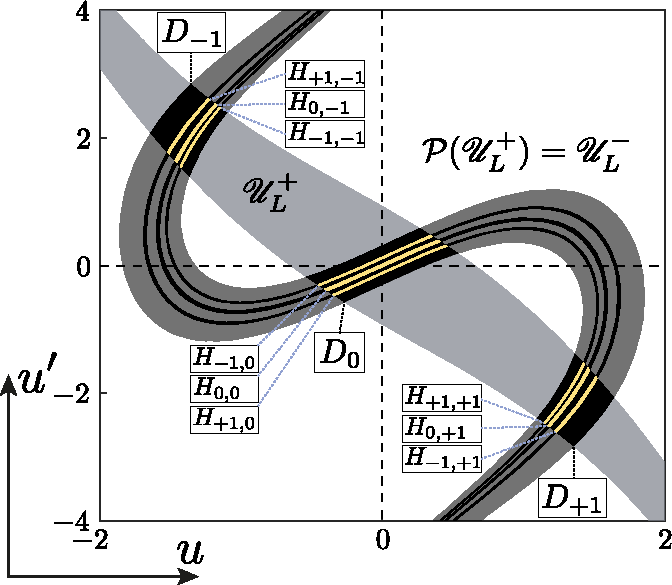
\includegraphics[scale = 1]{pic/h-strips for piecewise equation}
	\caption{
		Island set $\mathscr{U}_L = \mathscr{U}_L^+ \cap \mathscr{U}_L^-$ and sets $H_{ij} = \mathcal{P}(D_i) \cap D_j$, $i, j \in \{ -1, 0, +1 \}$ for equation \eqref{eq:stationary-piecewise} with parameters $(L_*, L_0) = (2, 1)$.
		Islands set $\mathscr{U}_L = \bigcup_{i \in S} D_i$ is forward-reachable, so $\mathcal{P}$-image of each island $D_i$ intersects all other islands $D_j$, $j \in S$ including $D_i$ itself.
	}
\label{fig:h-strips-piecewise}
\end{figure}

The similar illustration can be provided for $\mathcal{P}^{-1}$ map as well.
Island set $\mathscr{U}_L = \bigcup_{i \in S} D_i$ for Eq.~\eqref{eq:stationary-piecewise} is backward-reachable.
It means that $V_{ij} = \mathcal{P}^{-1}(D_i) \cap D_j \neq \varnothing$ for each $i, j \in S$.
On Figure~\ref{fig:v-strips-piecewise} sets $V_{ij}$ are depicted for $i, j \in \{ -1, 0, +1 \}$.

\begin{figure}[h]
\centering
	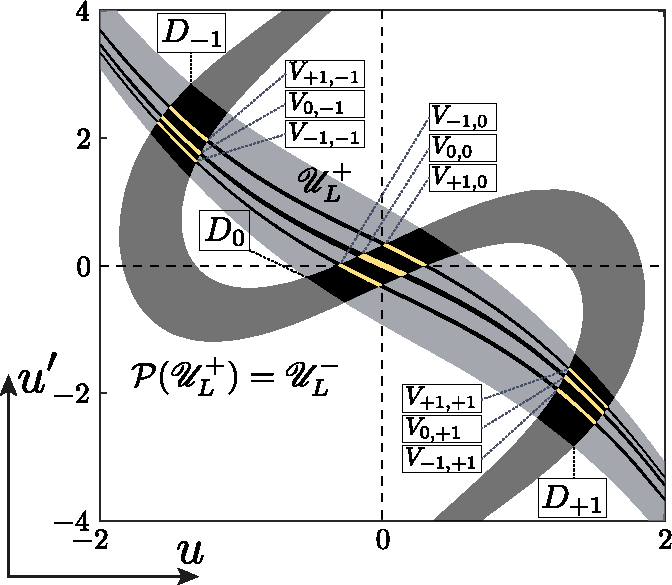
\includegraphics[scale = 1]{pic/v-strips for piecewise equation}
	\caption{
		Island set $\mathscr{U}_L = \mathscr{U}_L^+ \cap \mathscr{U}_L^-$ and sets $V_{ij} = \mathcal{P}^{-1}(D_i) \cap D_j$, $i, j \in \{ -1, 0, +1 \}$ for equation \eqref{eq:stationary-piecewise} with parameters $(L_*, L_0) = (2, 1)$.
		Islands set $\mathscr{U}_L = \bigcup_{i \in S} D_i$ is backward-reachable, so $\mathcal{P}$-pre-image of each island $D_i$ intersects all other islands $D_j$, $j \in S$ including $D_i$ itself.
	}
\label{fig:v-strips-piecewise}
\end{figure}

\section{Symbolic Dynamics: Solutions Coding}

In this sections we show how all the structures and properties introduced above can be used together to classify all bounded solutions of equation \eqref{eq:stationary}.
Our classification is closely connected with the structure of the $\mathscr{U}_L$ set.
We demonstrate our approach for the previously considered piecewise pseudopotential equation \eqref{eq:stationary-piecewise}.
Let's introduce two sets.

\begin{definition}
	Define set $\mathcal{O}$ as a set of all orbits of regular solutions for equation \eqref{eq:stationary}, i.e. $\{ \vb{p}_n \} \in \mathcal{O}$, $ \mathcal{P}(\vb{p}_n) = \vb{p}_{n+1}$, where $\mathcal{P}$ is a Poincar\'e map associated with equation \eqref{eq:stationary}.
\end{definition}

One can define a metric $\mathcal{O}$ as follows.
Let $v, w \in \mathcal{O}$ are two orbits, $v = \{ \vb{p}_n \}$, $\vb{p}_n = (\phi_n, \phi_n')$, $w = \{ \vb{q}_n \}$, $\vb{q}_n = (\psi_n, \psi_n')$, then the distance $d_{\mathcal{O}}$ between orbits $v$ and $w$ is defined as a Euclidean distance between points $\vb{p}_0$ and $\vb{q}_0$, i.e.
\begin{equation}
	d_{\mathcal{O}}(v, w) = ||\vb{p}_0 - \vb{q}_0 || = \sqrt{(\phi_0 - \psi_0)^2 + (\phi_0' - \psi_0')^2}.
\end{equation}
This implies that $\mathcal{O}$ can be regarded as a topological space where neighbourhood $U_{\varepsilon}(u^*)$ of an element $u^* \in \mathcal{O}$ is defined as $U_{\varepsilon}(u^*) = \{u \ | \ d_{\mathcal{O}}(u^*, u) < \varepsilon \}$.

\begin{definition}
	Define set $\mathcal{S}$ as a set of bi-infinite sequences $\{ \dots, i_{-1}, i_0, i_1, \dots \}$ over an alphabet where each symbol $i_k$, $k = 0, \pm 1, \dots$, corresponds to a connected component $D_k \in \mathscr{U}_L$.
\end{definition}

We also write $\mathcal{S}_N$ if the alphabet has $N$ different symbols, and $\mathcal{S}_{\infty}$ if the number of symbols is infinite (corresponds to the infinite number of connected components in $\mathscr{U}_L$).
Set $\mathcal{S}$ also can be regarded as a topological space where neighbourhood $W_k(\omega^*)$ of an element $\omega^* = \{ \dots, i_{-1}^*, i_0^*, i_1^*, \dots \} \in \mathcal{S}$ is defined as $W_k(\omega^*) = \{ \omega \ | \ i_s^* = i_s, |s| < k \}$.

What we are interested in is the connection between sets $\mathcal{O}$ and $\mathcal{S}$.
First of all the structure of island set $\mathscr{U}_L$ can be easily used to assign symbolic sequences, also named codes, to the solutions, so the correspondence from $\mathcal{O}$ to $\mathcal{S}$ can be trivially established.
Let's demonstrate it with an example.
Let one has a regular solution $u(x)$ of equation \eqref{eq:stationary-piecewise}.
Suppose that this is a localized solution depicted on Figure~\ref{fig:solution-and-orbit}~(a).
We inspect the values and the derivatives of the solution $u(x)$ in the points corresponding to the Poincar\'e sections associated with the period $L$, and then put these points $(u, u')$ onto the structure of the set $\mathscr{U}_L$ from the Panel~(b) of Figure~\ref{fig:solution-and-orbit}.
In the points $x = 0$ value and derivative $\vb{p}_0 = (u(0), u'(0))$ matches island $D_{-1}$.
After that in the point $x = L$ our solution $u(x)$ cross the central islands $D_0$ and matches it again for $x = 2L$.
In the point $x = 3L$ our solution came into the right island $D_{+1}$.
That allows us to determine four central symbols of the result code: $\{ -1, 0, 0, +1 \}$.
Moreover since our solution is localized all other points $(u(nL), u'(nL))$ correspond to the central component of $\mathscr{U}_L$ and all the symbols from the left side of ``$-1$'' and the right side of ``$+1$'' are ``$0$''.
So, finally we obtain the result bi-infinite sequence $\{ \dots, 0, -1, 0, 0, +1, 0, \dots \}$ for the localized solution $u(x)$ from Figure~\ref{fig:solution-and-orbit}~(a).
Obviously points of orbit of our solution cannot lie down outside of  $\mathscr{U}_L$ because the solution is regular and has bi-infinite orbit, so at each step we have exactly one symbol and the overall process identifies the result bi-infinite sequence uniquely.

% TODO: place dots exactly where they are on the Panel (b).
\begin{figure}[h]
\centering
	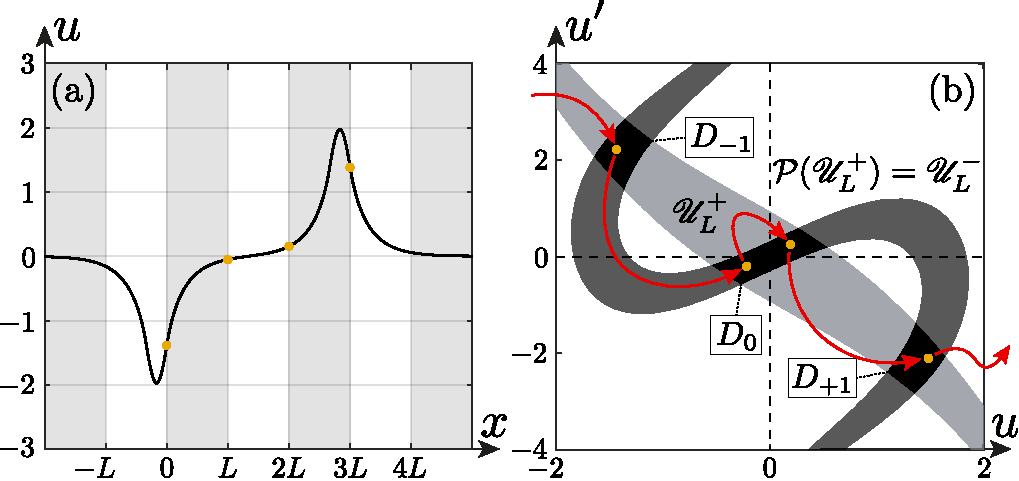
\includegraphics[scale = 1]{pic/solution and orbit on the phase plane}
	\caption{
		Illustration of the coding process.
		Panel~(a) represents a localized solution for the Eq.~\eqref{eq:stationary-piecewise} with parameters $(L_*, L_0) = (2, 1)$.
		This solution has been found numerically using the shooting method.
		Panel~(b) represents a sketch of four points (yellow dots) of the solution orbit over the structure of the $\mathscr{U}_L$ set.
		These points cross the islands accordingly to the red arrows and determine the symbols of the result solution code: $\{ \dots, 0, -1, 0, 0, +1, 0, \dots \}$.
	}
\label{fig:solution-and-orbit}
\end{figure}

\subsection{Uniqueness of Solutions Coding}

\section{Summary}